% TODO https://trello.com/
%
\chapter{Software Configuration Management}
In software engineering, software configuration management is the
task of tracking and controlling changes in the software, part of the
larger cross-disciplinary field of configuration management.
Software configuration management practices include revision control
and the establishment of baselines. If something goes wrong,
software configuration management can determine what was changed and
who changed it. If a configuration is working well, software configuration
management can determine how to replicate it across many hosts.
%Als Konfiguration eines Systems bezeichnet man die Festlegung seiner
%Elemente mit ihren Versionen resp. Varianten:
%(\href{http://www.software-kompetenz.de/?22704}
%{www.software-kompetenz.de/?22704})
\begin{quote}
A configuration is a defined stage of a product. This stage will contain
\begin{itemize}
\item Source code
\item Documentation
\item Config files
\item Tools
\item ... and all other specific things which are relevant for that product stage
\end{itemize}
%Eine Konfiguration ist ein Entwicklungsstand eines Produkts, in dem neben dem
%Quellcode und der Dokumentation sämtliche Werkzeuge und Hilfsmittel zum
%Erzeugen einer lauffähigen Version zusammengefasst sind. Das schließt auch die
%Dokumentation und die Einstellungen bzw. verwendete Parameter der Werkzeuge
%und Hilfsmittel ein.
\end{quote}
\newslide
There are several reasons why a software system is going through changes:
\begin{itemize}
\item New features
\item Bug fixes
\item New requirements
\item New libraries
\end{itemize}

%Softwaresysteme sind aus vielfältigen Gründen \"Anderungen unterworfen:
%Strategie- und Marketingentscheidungen, Fehlerbehebungen, Kundenforderungen,
%nicht mehr unterstützte Softwareversionen von Drittherstellern etc.

\newslide
%Änderungen betreffen meist unterschiedliche, von einander abhängige Elemente
Changes are affecting the following elements
\begin{itemize}
\item Requirements analysis
\item Design specification
\item Test specification
\item Project plan
\item Source code
\item Build files
\item 3rd party tools (Compiler, Libraries, Database \ldots)
\item User guide, operating guide
\item Training guide,
\item \ldots
\end{itemize}

Uncontrolled changes on one or more of these elements could finally end
up with software failures.\\

%Unkontrolliert durchgeführte Änderungen an einem oder mehreren Elementen
%können unversehends zu Funktionsstörungen oder anderen Inkonsistenzen
%führen.

Because of that, it is important to track every change in a software system
to ensure re-traceability.

%Deshalb: Um die Integrität und Rückverfolgbarkeit eines Softwaresystems zu
%gewährleisten, muss ein
%systematischer Änderungsprozess betrieben werden:
\begin{quote}
Configuration Management ... is a management process for establishing and
maintaining consistency of a product's performance, its functional and
physical attributes, with its requirements, design and operational
information, throughout its life. (ANSI/EIA)
\end{quote}
\newpage
\section{Classification (IEEE/SWEBOK)}
\begin{figure}[H]
\centering
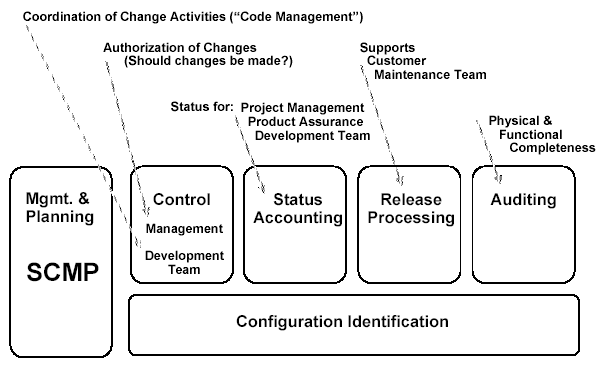
\includegraphics[width=0.75\linewidth]{config-management/scm-activities}
\caption{Software Configuration Management (Source: SWEBOK)}
\end{figure}
\begin{itemize}
\item \underline{SCMP}
   (Management des Software-Konfigurationsprozesses):
  \begin{itemize}
  \item Organisatorischer Kontext: Einbindung in die betriebliche
  Organisation, Bezeichnung der Schnittstellen und Verantwortlichkeiten,
\item Randbedingungen und Wegleitung: Berücksichtigung juristischer,
  ökonomischer, unternehmenspolitischer Faktoren, Anwendung von
  ``Best-Practices''
\item Planung: Festlegung und Anpassung der Verfahren und Werkzeuge zur
  Identifikation der Software-Elemente, Steuerung und Überwachung des
  Prozesses, Release-Management und Auslieferung, unter Berücksichtigung des
  Projektumfanges
  \end{itemize}
\item \underline{Configuration Identification}:
  Software configuration identification identifies items to be
  controlled, establishes identification schemes for the items and
  their versions, and establishes the tools and techniques to be
  used in acquiring and managing controlled items. These activities
  provide the basis for the other software configuration management
  activities.
  %Festlegung und Beschreibung Software configuration status accounting (SCSA) is an element of configuration management consisting of the recording and reporting of information needed to manage a configuration effectively. der Bezugskonfiguration (Baseline),
  %Markierung der Elemente, Aufnahme in die Konfiguration,
  %Zulassungsverfahren (approval), Bezeichnung der Software-Bibliotheken
\item \underline{Control}:
  Software configuration control is concerned with managing changes
  during the software life cycle. It covers the process for
  determining what changes to make, the authority for approving certain
  changes, support for the implementation of those changes,
  and the concept of formal deviations from project requirements as
  well as waivers of them. Information derived from these activities
  is useful in measuring change traffic and breakage as well as aspects
  of rework.
  %formelle Organisation und Behandlung von Änderungen,
  %Strukturierung der Anfragen (Requests), Abschätzung der Auswirkungen,
  %Durchführung und Freigabe, Umgang mit Abweichungen (Verzichtserklärungen)
\item \underline{Status Accounting}:
  Software configuration status
  accounting (SCSA) is an element of configuration management
  consisting of the recording and reporting of information needed to
  manage a configuration effectively.
%Aufzeichnung der Aktivitäten mit
%  Terminangaben und
%  kommentierenden Erläuterungen, Ablageverfahren, Berichterstattung
\item \underline{Auditing}:
  A software audit is an independent examination of a work product or set
  of work products to assess compliance with specifications, standards,
  contractual agreements, or other criteria.
  %Einhaltung der Vorgaben,
  %Durchführung von Audits
%Evaluation von Verbesserungen
\item \underline{Release Processing}:
  Release processing refers to the distribution of a software
  configuration item outside the development activity; this includes
  internal releases as well as distribution to customers.
  %Festlegung,
  %Erstellung und
  %Beschreibung der auszuliefernden Konfiguration (Release Notes: neue
  %Funktionalität, bekannte
  %Einschränkungen und Probleme, Plattform-Anforderungen), Mitteilung an Kunden
\end{itemize}
%\newpage
%----------------------------------------------------------------------
\section{Versionen, Revisionen und Ausgaben}
Ein File (Dokument) kann verschiedene Versionen haben:
\begin{figure}[H]
\begin{center}
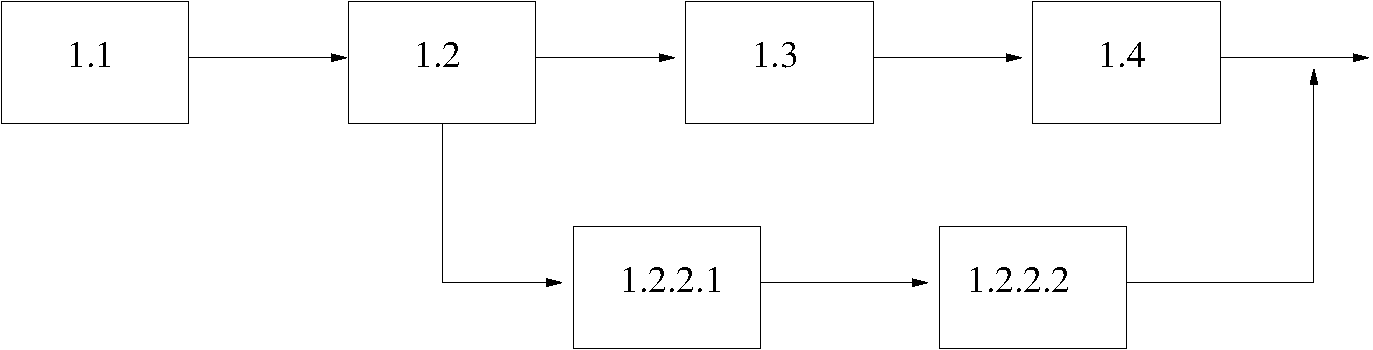
\includegraphics[width=0.8\linewidth]{config-management/xfig/file-revisions}
\end{center}
\caption{Die Versionen einer Datei}
\end{figure}
Sie werden \underline{Revisionen} (engl. Revisions) genannt.

\ifslides
\else
Ebenso kann ein Softwareprodukt mehrere Versionen haben. Man
nennt sie \underline{Ausgaben} (engl. Releases). Ihre Sourcefiles
haben jedoch unterschiedliche Versionen:

\fi
\begin{figure}[H]
\begin{center}
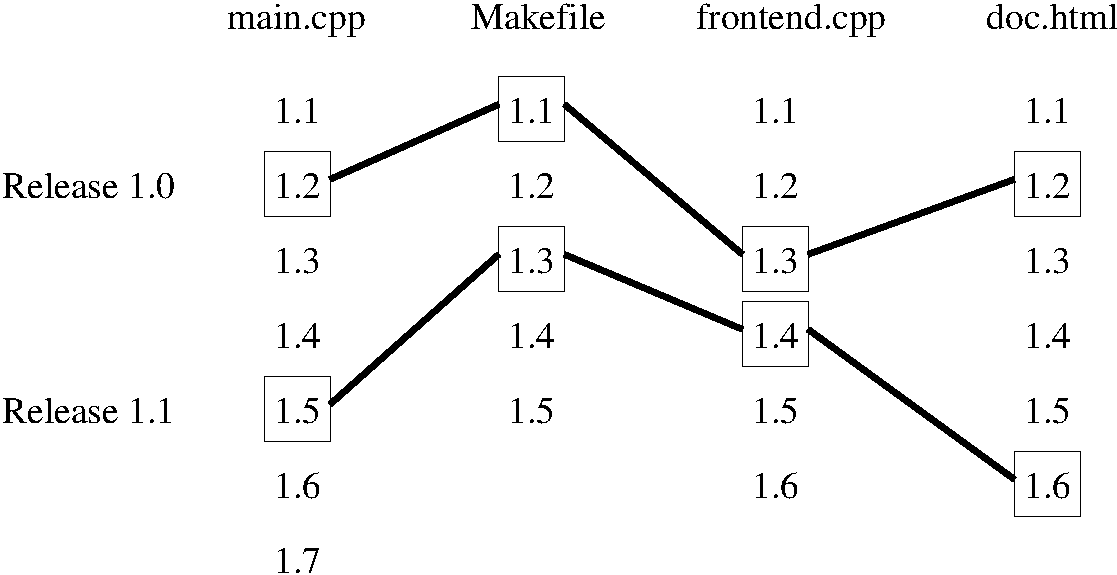
\includegraphics[width=0.9\linewidth]{config-management/xfig/releases}
\end{center}
\caption{Die Versionen eines Produktes}
\end{figure}
\newslide

Die Entwicklung erfolgt normalerweise entlang des Hauptastes
(Trunk oder Master). In mehreren Zyklen werden Dateien modifiziert,
hinzugefügt, gelöscht und umbenennt.

Bevor ein neuer Release gebildet wird, empfiehlt es sich
eine Verzweigung (Branch) zu erstellen. Dieser Moment wird auch als
``Code'' resp. ``Feature freeze'' bezeichnet, da innerhalb dieser Verzweigung
keine funktionalen Erweiterungen sondern nur noch diejenigen
Änderungen durchgeführt werden, die für die Integrations- und
Systemtests nötig sind. Nach Abschluss dieser Phase sollten die
Änderungen wieder mit dem Hauptast zusammengeführt werden.
\begin{figure}[H]
\begin{center}
  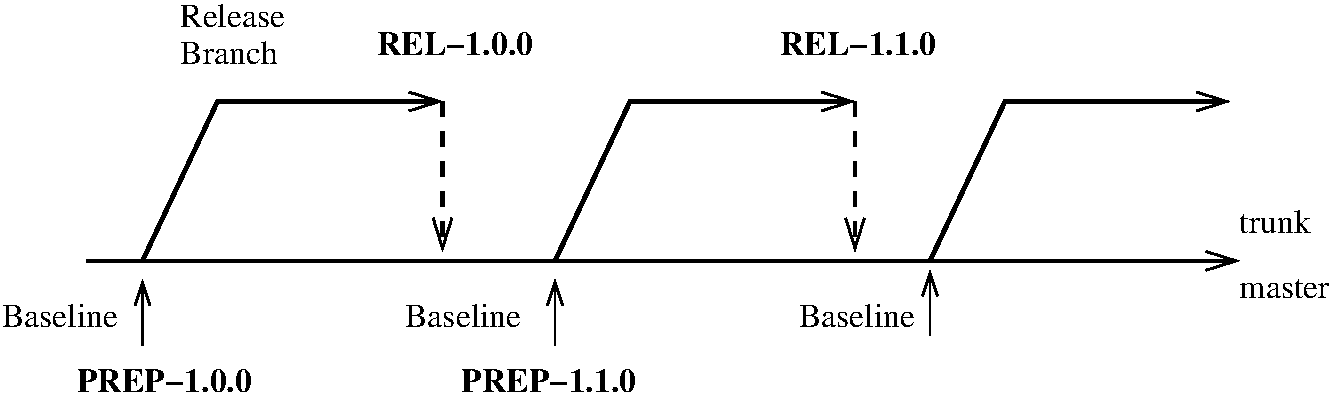
\includegraphics[width=0.9\linewidth]{config-management/xfig/release-branch}
\end{center}
\caption{Release-Bildung mit Branches und Merges}
\end{figure}
Die nicht mit dem Release beschäftigten Entwickler können während der
Release-Bildung auf dem Trunk weiterarbeiten.

\newslide
Für die Release-Bezeichnung empfiehlt es sich, ein einfaches und
nachvollziehbares Schema
anzuwenden. Z. B: {\bfseries major.minor.patch}

\begin{tabular}{ll}
Major: & umfangreiche Änderungen oder Erweiterungen\\
Minor: & zusätzliche Funktionalitäten\\
Patch: & Fehlerbehebungen oder geringfügige Verbesserungen\\
\end{tabular}

% Siehe http://apr.apache.org/versioning.html
%---------------------------------------------------------------
\newpage
%\subsection*{Konfigurationsmanagement}
\section{Change Management}
\begin{figure}[H]
\ifslides
\begin{center}
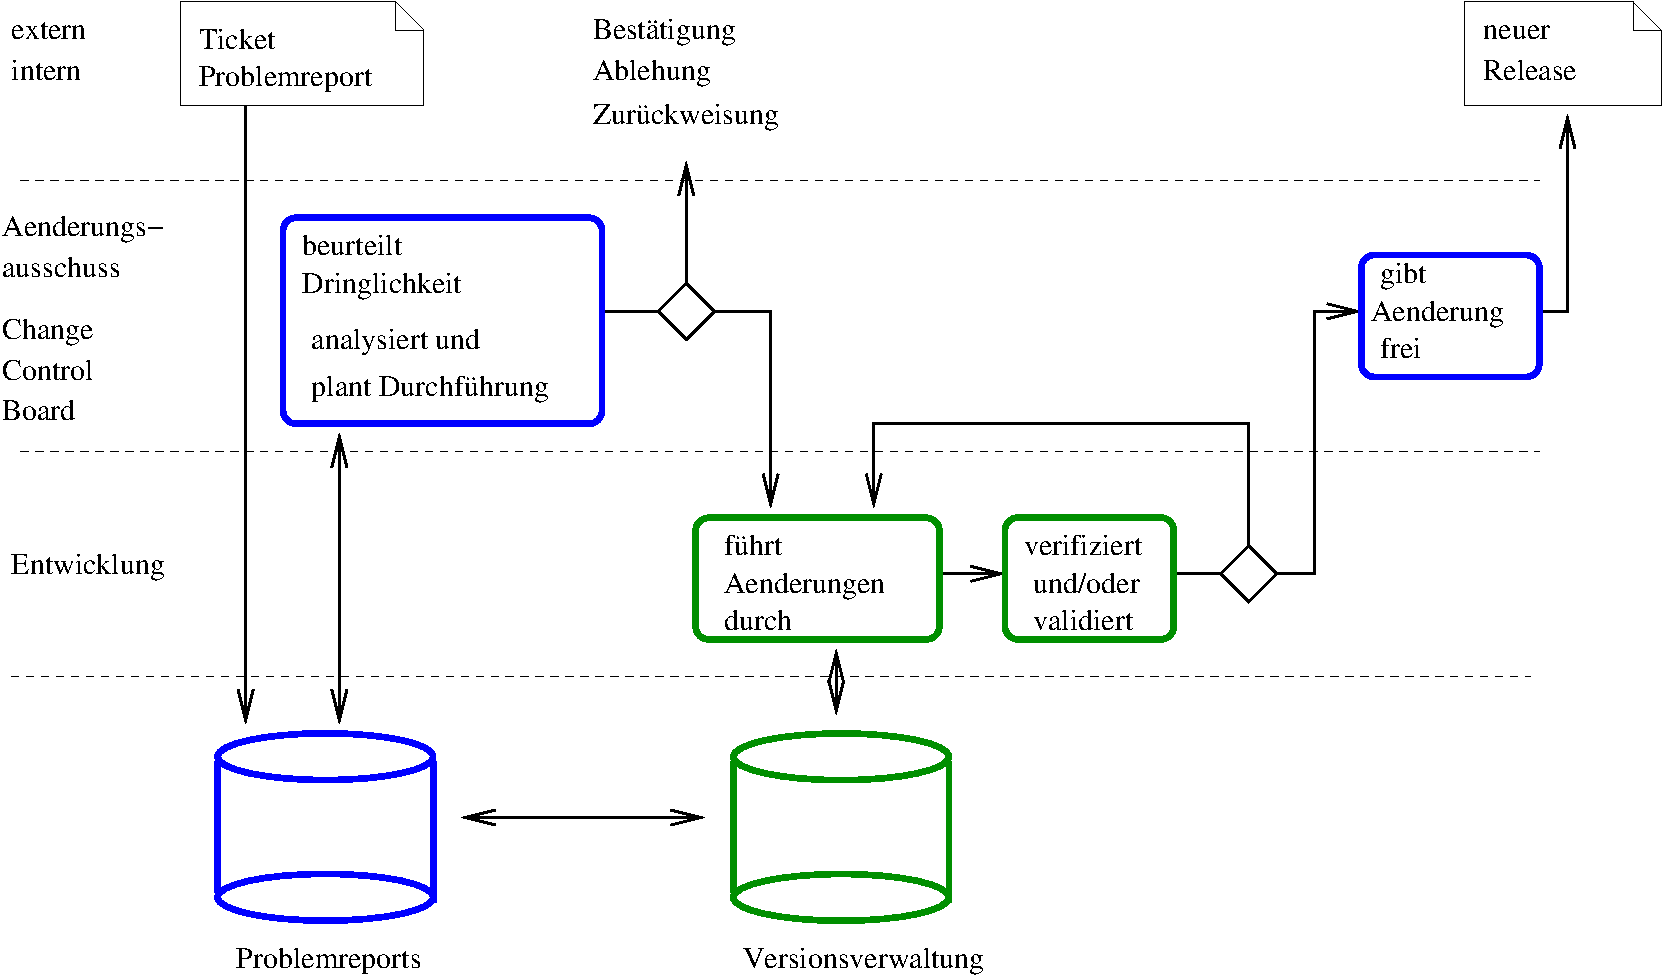
\includegraphics[width=0.65\linewidth]{config-management/xfig/changemgmt}\\[2ex]
\end{center}\else
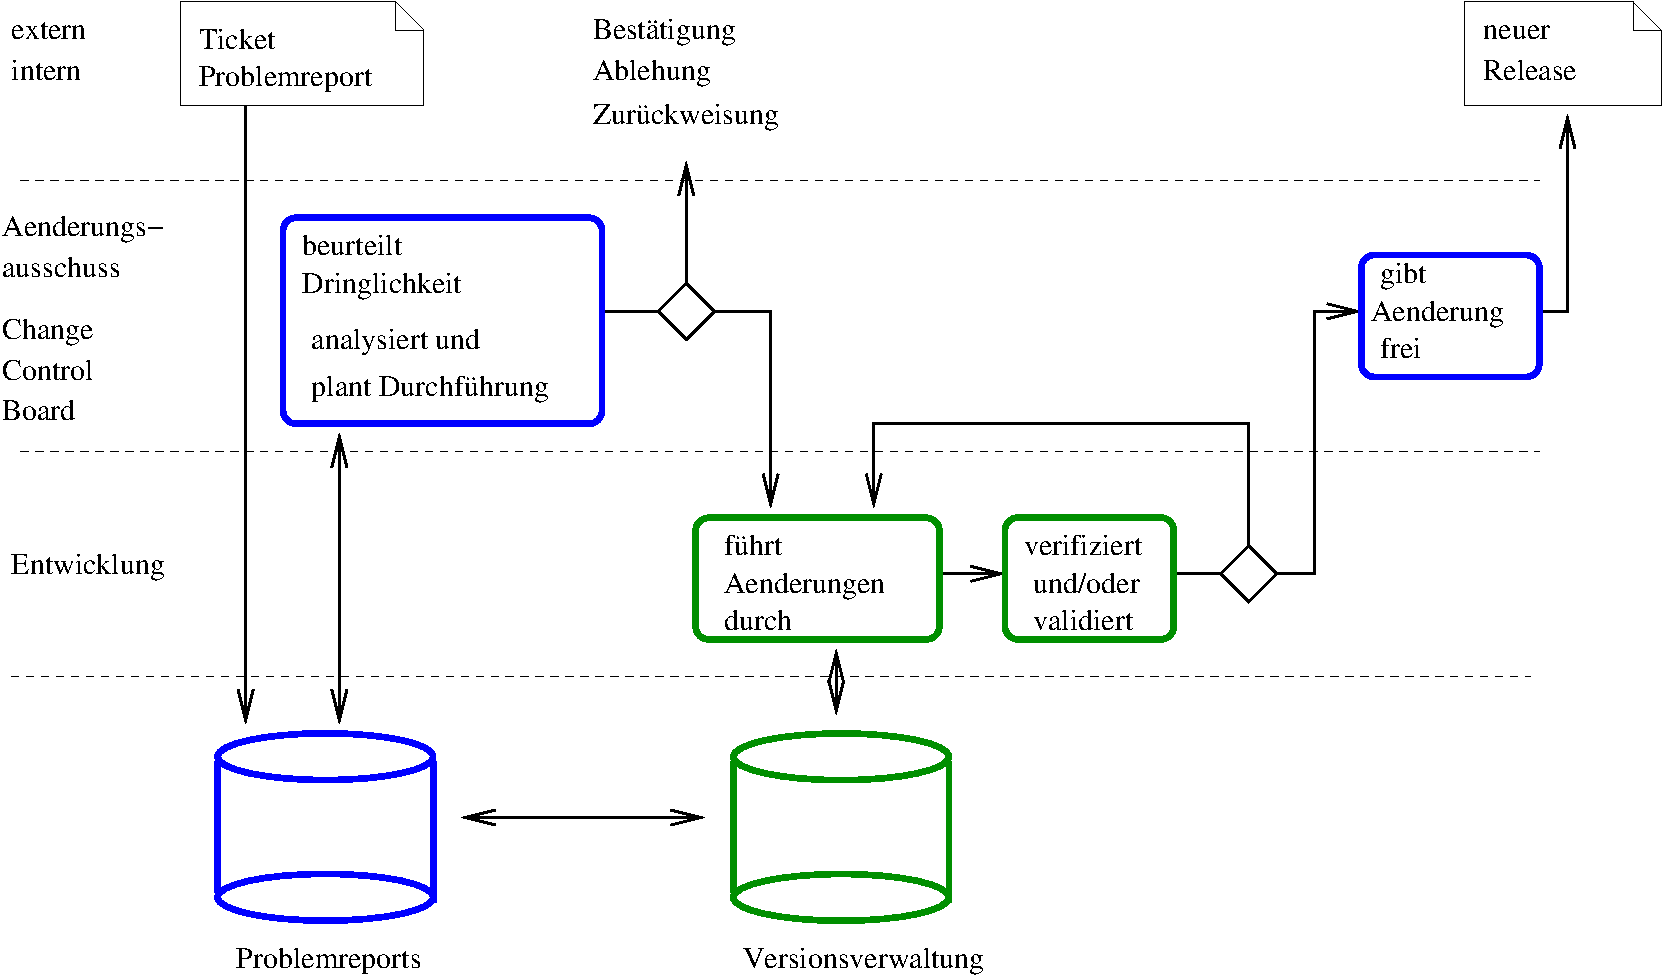
\includegraphics[width=\linewidth]{config-management/xfig/changemgmt}
\caption{Der Änderungsprozess}
\fi
\end{figure}
\begin{minipage}[t]{0.48\linewidth}
\subsection*{Bug and Issue Tracking} %Problembehandlung
\begin{itemize}
\item Erfassung und Verwaltung aller eingehender Fehlermeldungen
  und \"Anderungsanträgen
\item Entscheidung über die Bearbeitung der Meldungen unter Berücksichtigung
 der technischen und zeitlichen Auswirkungen
\item Abschluss der \"Anderung und Information der Betroffenen
\end{itemize}
\end{minipage}
\hfill
\begin{minipage}[t]{0.48\linewidth}
\subsection{Version Control}
\begin{itemize}
\item Eindeutige Kennzeichnung der Software-Elemente
\item Einfrieren von Zwischenergebnissen
\item Sicherstellen dass auf vorangegangene Versionen
  zurückgegriffen werden kann
\end{itemize}
\end{minipage}
\newslide
\section{Software and further Informations}
\begin{itemize}
\item Software Engineering Body of Knowledge (Kap. 7 SCM):
  \href{http://www.swebok.org}{www.swebok.org}
\item Eine nützliche  Linksammlung: \href{http://www.cmcrossroads.com/yp}
                                          {www.cmcrossroads.com/yp/}
\end{itemize}
%---------------------------------------------------------------
\newslide
% CRISP: Complete Repeatable Informative Schedulable Portable
% (Pragmatic Project Automation)
%
